\begin{figure}
\centering	
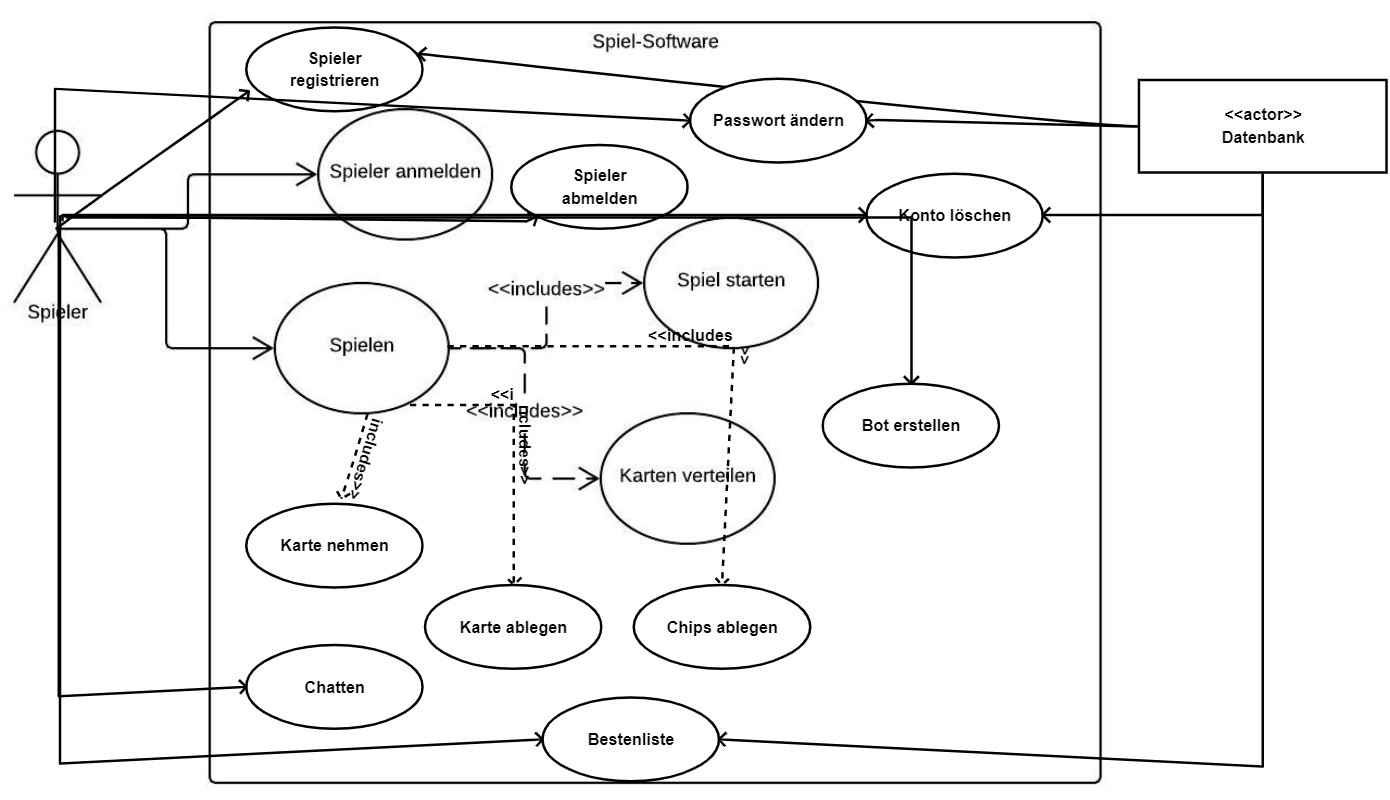
\includegraphics[width=0.9\textwidth]{img/ucd.png}
\label{fig:sys}
\caption{Systemgrenzendiagramm}
\end{figure}

\section{Systemgrenze (Use Case Diagramm)}

Die Systemgrenze wird in der Abbildung~\ref{fig:sys} dargestellt\footnote{Weitere Erklärungen und Spezifizierungen, die sich auf Abgrenzungen der Verantwortlichkeiten vom System und weiteren Akteuren/Systemen beziehen, können hier spezifiziert werden.}. 


\section{Beschreibungen der Anwendungsfälle}


\newcounter{uc}\setcounter{uc}{10}

\begin{description}[leftmargin=5em, style=sameline]

	\begin{lhp}{uc}{UC}{uc:registrieren}
		\item [Name:]Spieler registrieren. 
		\item [Ziel:] Spieler registriert sich ins System.
		\item [Akteure:] Spieler und Datenbank.
		\item [Vorbedingungen:] Der Spieler befindet sich noch nicht in einem Raum
		\item [Eingabedaten:] Zugriffsdaten. Mit Referenzen auf~\ref{section:productdaten}.
		\item [Beschreibung:] Spieler registriert sich.
		\item [Ausnahmen:] \textit{Falls der eingegebene Benutzername schon vergeben ist: } zeigt das System eine Fehlermeldung an.
		\item [Ergebnisse und Outputdaten:] Nach der erfolgreiche Registrierung,ist der Spieler in der Lobby und hat zugriff auf Bestenliste und Räume.
		\item [Systemfunktionen] \ref{funk:zugriff}
	\end{lhp}
	
	\begin{lhp}{uc}{UC}{uc:anmelden}
		\item [Name:] Spieler anmelden.
		\item [Ziel:] Spieler meldet sich im System an.
		\item [Akteure:] Spieler und Datenbank.
		\item [Vorbedingungen] Spieler ist im Vorraum.
		\item [Eingabedaten:] Zugriffsdaten~\ref{daten:benutzername}~\ref{daten:passwort}.
		\item [Beschreibung:] Spieler meldet sich an.							
		\item [Ausnahmen:] \hfill
			\begin{itemize} 
				\item[] \textit{Passwort oder Benutzername ist falsch:} Das System zeigt eine Fehlermeldung an, anstatt des Schrittes 2.
				
			\end{itemize}
		\item [Ergebnisse und Outputdaten:] Spieler ist in der Lobby und sieht die Bestenliste.	
		\item [Systemfunktionen:] \ref{funk:zugriff}.
	\end{lhp}
	
	
		\begin{lhp}{uc}{UC}{uc:abmelden}
		\item [Name:] Spieler abmelden.
		\item [Ziel:] Spieler meldet sich aus dem System aus.
		\item [Akteure:] Spieler.
		\item [Vorbedingungen] Spieler ist in der Lobby und angemeldet.
		\item [Eingabedaten:] Keine.
		\item [Beschreibung:] Spieler meldet sich ab.
		\item [Ausnahmen:] Keine.
		\item [Ergebnisse und Outputdaten:] Spieler ist im Vorraum, Spieler wurde abgemeldet.	
		\item [Systemfunktionen:] \ref{funk:zugriff}.
	\end{lhp}
	
	
	\begin{lhp}{uc}{UC}{uc:löschen}
		\item [Name:] Konto löschen.
		\item [Ziel:] Spieler entfernt seine Daten aus dem System.
		\item [Akteure:] Spieler.
		\item [Vorbedingungen] Spieler ist im Vorraum.
		\item [Eingabedaten:] Passwort~\ref{daten:passwort}.
		\item [Beschreibung:] Spieler löscht das eigene Konto komplett.
		\item [Ausnahmen:] \hfill
			\begin{itemize} 
			\item[] \textit{Passwort ist falsch:} Das System zeigt eine Fehlermeldung an, anstatt des Schrittes 2.
			\item[] \textit{Keine Löschung erwünscht:} Anstatt des Schrittes 4, schließt das System den Dialog.				
			\end{itemize}
		\item [Ergebnisse und Outputdaten:] Spieler ist im Vorraum, Spielerkonto wurde gelöscht.	
		\item [Systemfunktionen:] \ref{funk:zugriff}.
	\end{lhp}

	\begin{lhp}{uc}{UC}{uc:chatten}
		\item [Name:] Chatten.
		\item [Ziel:] Spieler sendet und liest Nachrichten.
		\item [Akteure:] Spieler.
		\item [Vorbedingungen] Spieler ist angemeldet und in der Lobby oder in einem Spielraum.
		\item [Eingabedaten:] Keine.
		\item [Beschreibung:] Spieler chattet mit anderen Spielern.
		\item [Ausnahmen:] \hfill
		\begin{itemize} 
			\item[] \textit{Die gesendete Nachricht ist zu lang :} Das System zeigt eine Fehlermeldung an			
		\end{itemize}
		\item [Ergebnisse und Outputdaten:] Spieler liest entweder Nachrichten oder sendet eine, welche dann im Chat zu sehen ist. 	
		\item [Systemfunktionen:] \ref{funk:chat}.
	\end{lhp}


	\begin{lhp}{uc}{UC}{uc:bestenliste}
		\item [Name:] Bestenliste.
		\item [Ziel:] Spieler werden in der Bestenliste angezeigt.
		\item [Akteure:] Spieler.
		\item [Vorbedingungen] Spieler ist in der Lobby.
		\item [Eingabedaten:] 
		\item [Beschreibung:] Spieler schaut sich die Bestenliste an.
		\item [Ausnahmen:] Keine.
		\item [Ergebnisse und Outputdaten:] Dem Spieler wird dynamisch die Bestenliste angezeigt	
		\item [Systemfunktionen:] \ref{funk:bestenliste}.
	\end{lhp}

	\begin{lhp}{uc}{UC}{uc:spielraum erstellen}
		\item [Name:] Spielraum erstellen.
		\item [Ziel:] Spieler erstellt einen Spielraum.
		\item [Akteure:] Spieler.
		\item [Vorbedingungen] Spieler ist in der Lobby.
		\item [Eingabedaten:] Keine.
		\item [Beschreibung:] Spieler erstellen eine Spielraum mit einer kapazität um mit anderen zu spielen.
		\item [Ausnahmen:] \hfill
		\begin{itemize} 
			\item[] \textit{Spielraum Name existiert bereits:} Das System zeigt eine Fehlermeldung an.
			
		\end{itemize}
		\item [Ergebnisse und Outputdaten:] Spieler ist im erstellten Spielraum.	
		\item [Systemfunktionen:] \ref{funk:spielraum}.
	\end{lhp}

		\begin{lhp}{uc}{UC}{uc:spielraum eintreten}
		\item [Name:] Spielraum eintreten.
		\item [Ziel:] Spieler tretet einem Spielraum ein.
		\item [Akteure:] Spieler.
		\item [Vorbedingungen] Spieler ist in der Lobby.
		\item [Eingabedaten:] Keine.
		\item [Beschreibung:] Spieler tretet einem Spielraum ein um mit anderen zu spielen
		\item [Ausnahmen:] \hfill
		\begin{itemize} 
			\item[] \textit{Spielraum ist bereits voll:} Das System zeigt eine Fehlermeldung an.
			
		\end{itemize}
		\item [Ergebnisse und Outputdaten:] Spieler ist im gewollten Spielraum.	
		\item [Systemfunktionen:] \ref{funk:spielraum}.
	\end{lhp}


	\begin{lhp}{uc}{UC}{uc:spielraum verlassen}
		\item [Name:] Spielraum verlassen.
		\item [Ziel:] Spieler verlässt einen Spielraum.
		\item [Akteure:] Spieler.
		\item [Vorbedingungen] Spieler ist in einem Spielraum
		\item [Eingabedaten:] Keine.
		\item [Beschreibung:] Spieler verlässt einen Spielraum.
		\item [Ausnahmen:] Keine
		\item [Ergebnisse und Outputdaten:] Spieler verlässt den Spielraum in dem er sich befand und ist zurück in der Lobby.	
		\item [Systemfunktionen:] \ref{funk:spielraum}.
	\end{lhp}

	\begin{lhp}{uc}{UC}{uc:spielen}
		\item [Name:] Spielen.
		\item [Ziel:] Spieler startet eine Runde Kings in the Corner mit anderen Spielern.
		\item [Akteure:] Spieler.
		\item [Vorbedingungen] Spieler befindet sich in einem Spielraum.
		\item [Eingabedaten:] Keine.
		\item [Beschreibung:] Sobald die benötigte Anzahl von Spielern erreicht ist, dann kann das Spiel starten. 
		\item [Ausnahmen:] \hfill
		\begin{itemize} 
			\item \textit{ Ist die minimale Anzahl von Spielern nicht erreicht:} zeigt das System eine Fehlermeldung.
		\end{itemize}
		\item [Ergebnisse und Outputdaten:] Eine Runde Kings in the Corner wird gestartet.  
		\item [Systemfunktionen:] \ref{funk:spielverw}.
	\end{lhp}

	\begin{lhp}{uc}{UC}{uc:karte legen}
		\item [Name:] Karte ablegen.
		\item [Ziel:] Spieler legt Karten ab.
		\item [Akteure:] Spieler.
		\item [Vorbedingungen] Spieler ist in einer laufenden Spielrunde.
		\item [Eingabedaten:] Keine.
		\item [Beschreibung:] Spieler legt eine Handkarte ab
		\item [Ausnahmen:] \hfill
		\begin{itemize} 
			\item[] \textit{Es wird gegen die Spielregeln verstoßen:} Das System zeigt eine Fehlermeldung an.
			
		\end{itemize}
		\item [Ergebnisse und Outputdaten:] Die abgelegte Karte liegt auf dem Tabbedstalll.
		\item [Systemfunktionen:] \ref{funk:spielverw}.
	\end{lhp}

	\begin{lhp}{uc}{UC}{uc:karte nehmen}
		\item [Name:] Karte nehmen.
		\item [Ziel:] Spieler nimmt eine Karte.
		\item [Akteure:] Spieler.
		\item [Vorbedingungen] Spieler ist in einem laufenden Spiel.
		\item [Eingabedaten:] Keine.
		\item [Beschreibung:] Spieler nimmt eine Karte vom Stapel.
		\item [Ausnahmen:] \hfill
		\begin{itemize} 
			\item
		\end{itemize}
		\item [Ergebnisse und Outputdaten:] Die gezogene Karte wird auf der Spielhand  angezeigt.
		\item [Systemfunktionen:] \ref{funk:spielverw}.
	\end{lhp}

	\begin{lhp}{uc}{UC}{uc:chips ablegen}
		\item [Name:] Chips ablegen.
		\item [Ziel:] Spieler legt Chips ab.
		\item [Akteure:] Spieler.
		\item [Vorbedingungen] Spieler ist in einer laufenden Spielrunde.
		\item [Eingabedaten:] Keine.
		\item [Beschreibung:] Spieler legt Chips ab
		\item [Ausnahmen:] \hfill
		\begin{itemize} 
			\item[] \textit{Es wird gegen die Spielregeln verstoßen:} Das System zeigt eine Fehlermeldung an.
			
		\end{itemize}
		\item [Ergebnisse und Outputdaten:] Die Chips werden vom Spieler abgelegt .
		\item [Systemfunktionen:] \ref{funk:spielverw}.
	\end{lhp}


	\begin{lhp}{uc}{UC}{uc:bots}
		\item [Name:] Bot erstellen.
		\item [Ziel:] Spieler fügt Bots zum Spiel hinzu.
		\item [Akteure:] Spieler.
		\item [Vorbedingungen] Spieler ist der Ersteller des Spielraums und befindet sich in diesem.
		\item [Eingabedaten:] Keine.
		\item [Beschreibung:] Spieler fügt Bots zum Spiel hinzu, falls ein Spieler den Raum verlässt.
		\item [Ausnahmen:] \hfill
		\begin{itemize} 
			\item
		\end{itemize}
		\item [Ergebnisse und Outputdaten:] Der erstellte Bot wurde dem Spiel hinzugefügt.	
		\item [Systemfunktionen:] \ref{funk:bots}.
	\end{lhp}
	
	\begin{lhp}{uc}{UC}{uc:daten prüfen}
		\item [Name:] Daten prüfen.
		\item [Ziel:] Die Datenbank überprüft die gegebenen Daten.
		\item [Akteure:] Datenbank.
		\item [Vorbedingungen] Spieler führt eine der Aktionen \ref{uc:registrieren}, \ref{uc:anmelden}, \ref{uc:löschen} aus.
		\item [Eingabedaten:] Zugriffsdaten~\ref{daten:benutzername}~\ref{daten:passwort}~\ref{daten:geburtsdatum}.
		\item [Beschreibung:] Spieler möchte sich anmelden, registrieren oder seinen Account löschen. Daraufhin überprüft die Datenbank die gegebenen Daten.
		\item [Ausnahmen:] \hfill
		\begin{itemize} 
				\item[] \textit{Daten sind nicht im Datenbanksystem vorhanden:} Die Datenbank gibt eine Rückmeldung ans System das die Daten nicht existieren.
				
			\end{itemize}
		\item [Ergebnisse und Outputdaten:] Falls Daten Korrekt sind wird die gewollte Aktion ausgeführt, wenn nicht wird eine Fehlermeldung zurückgegeben.	
		\item [Systemfunktionen:] \ref{funk:zugriff}.
	\end{lhp}



\end{description}